\scanpage{14}
\figure{
\begin{tikzpicture}[x=0.65cm,y=0.65cm]
\draw[red,line width=2pt,rounded corners=2pt] (0,0) rectangle (16,11);
\draw[blue,line width=2pt,rounded corners=2pt] (.2,.2) rectangle (15.8,10.8);
\end{tikzpicture}}

\figure{
\begin{tikzpicture}[x=0.7cm,y=0.7cm]
\node[align=left,anchor=west] at (0,2.6) {of\\Science};
\draw[red] (0,.7)--(.2,1.1)--(.9,.95)..controls (1.7,1.2) and (2.05,2.1)..(2.2,3)--(2.6,3.1)..controls (3,2.3) and (2.4,1.3)..(1.7,.65)--(.1,.6)--(0,.7);
\draw[red] (0,.55)--(.8,.55)--(.9,.35)--(0,.35);
\draw[red] (1.6,.65)--(2.9,1.2)--(3.3,.75)--(2,.55);
\draw[red] (1.6,.8)--(2.9,1.35) (1.75,.7)--(3.1,1.03) (1.8,.55)--(3.3,.78);
\draw[red] (2.2,3)--(2.05,3.55) (2.3,3)--(2.3,3.6) (2.4,3)--(2.55,3.6) (2.55,3.05)--(2.8,3.55);
\foreach \x/\y in {1/.8,1.3/.9,1.6/1,1.9/1.2,2.1/1.4,2.3/1.6,2.4/1.9,2.5/2.2,2.4/2.5,2.4/2.8,1.4/.65,1.7/.75,2/1,2.2/1.2,2.5/1.5,2.6/1.8,2.6/2.1,2.6/2.4,2.6/2.7} {\draw[red] (\x,\y) circle (.06);}
\node at (1.7,0) {NAGOYA UNIV.};
\end{tikzpicture}}
% crop-candidate: scan 14

\figure{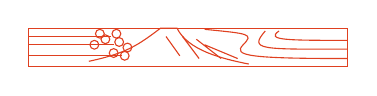
\begin{tikzpicture}[x=.7cm,y=.7cm]
\draw[red!50!brown] (0,0) rectangle (5.8,.7);
\draw[red!50!brown] (0,.2)--(1.7,.2) (0,.4)--(1.55,.4) (0,.55)--(1.5,.55);
\draw[red!50!brown] (1.1,.1)..controls(1.8,.25)and(2,.4)..(2.4,.7)--(2.7,.7)..controls(2.9,.3)and(3.5,.15)..(4,.05);
\draw[red!50!brown] (2.5,.55)--(2.75,.2) (2.8,.55)--(3.1,.15) (3.05,.5)--(3.5,.15) (3.2,.4)--(3.8,.15);
\draw[red!50!brown] (3.2,.68)..controls(4,.6)and(4.1,.6)..(3.9,.4)..controls(3.7,.2)and(4,.15)..(5.8,.15);
\draw[red!50!brown] (4.3,.65)..controls(4,.3)and(4.2,.32)..(5.8,.32);
\draw[red!50!brown] (4.55,.65)..controls(4.3,.48)and(4.7,.48)..(5.8,.48);
\foreach \x/\y in {1.2/.4,1.4/.5,1.65/.45,1.8/.35,1.55/.25,1.75/.2,1.3/.6,1.6/.6} {\draw[red!50!brown] (\x,\y) circle (.08);}
\end{tikzpicture}}
% crop-candidate: scan 14

\diagram{\begin{array}{|c|c|c|}\hline
& & \text{\unsure{日本郵便}}\\\hline
20.12.77&\begin{gathered}\text{名古屋大学内}\\\text{NAGOYA DAIGAKUNAI}\\\text{JAPAN}\end{gathered}&0,340\\\hline
\end{array}}
HI208

Professeur Alexandre Grothendieck

34700 Villecun (Lodève)

\uline{FRANCE}

VIA AIR MAIL\\
PAR AVION

\diagram{\begin{array}{|c|}\hline
\text{PAR AVION}\\
\text{航空郵便}\\\hline
\end{array}}

\margin{\unsure{340}}

$\{\lambda,\lambda^{-1}\}\qquad |\lambda|\ne1$

$\lambda+\lambda^{-1}=\alpha\qquad\deleted{\unsure{ssi}}\quad\alpha\notin[-2,+2]$

$\alpha^2-4$

$\unsure{\Leftrightarrow}\lambda\bar\lambda=1$\\
$\bar\lambda=\lambda^{-1}$\\
$\lambda+\lambda^{-1}$ \uline{réel}

Donc $\lambda\ne\lambda^{-1}$ i.e. $\lambda^2\ne1$ i.e. $\lambda\ne\pm1$ i.e. $\alpha\ne\pm2$
% archive foliation: 13
